
%%%%%%%%%%%%%%%%
% Segmentation %
%%%%%%%%%%%%%%%%

\section{Segmentation}
\label{sec:segm}



% Binary segmentation network %
%%%%%%%%%%%%%%%%%%%%%%%%%%%%%%%


\subsection{Binary segmentation network}
\label{sec:segm_1}

This section\footnote{The code for this section is found at \texttt{scripts/itnodl\_segm.py}.
} discusses a deep convolutional binary segmentation network, based largely on the autoencoder described in section \textcolor{blue}{\ref{sec:auto2}}. To train the model, a subset of the full dataset was used (see section \textcolor{blue}{\ref{sec:intro}} for details). In accordance with the assignment, training labels were binarized. This was accomplished by converting the segmented images to grayscale and applying a threshold of .02 to the pixel values. This made sure that only the black pixels remained $0$, and all the others were set to $1$. Throughout this section, I'll refer to the 1-values as 'foreground', and the 0-values as 'background'.

\begin{figure}[!htbp]
  \begin{center}
    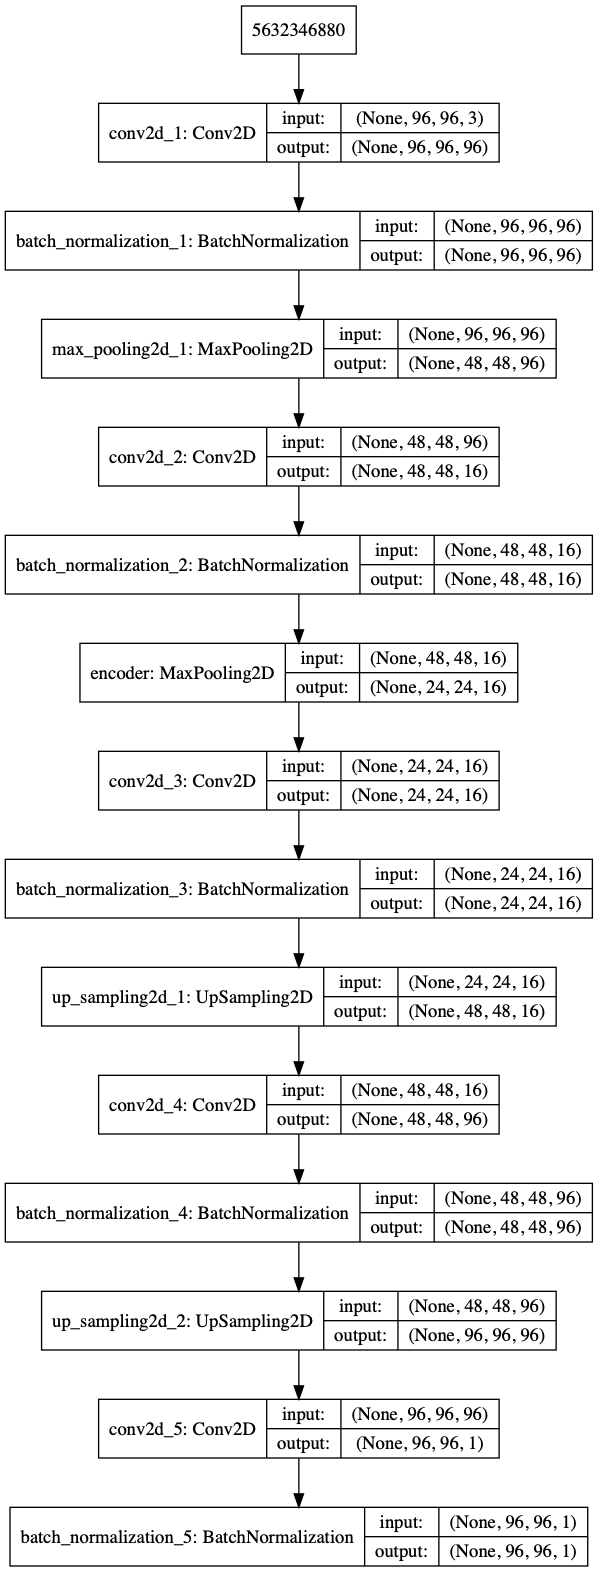
\includegraphics[height=18cm, keepaspectratio]{images/segm_architecture}
    \caption{Deep convolutional architecture for the segmentation network. Input dimensions are $96 \times 96 \times 3$. The model predicts a score per pixel position, ignoring color channels---hence the output dimensions are $96 \times 96 \times 1$.}
    \label{fig:segm_architecture}
  \end{center}
\end{figure}

\paragraph{Architecture} The architecture of the segmentation network is shown in \ref{fig:segm_architecture}. It is very closely related to the DCA architecture (see figure \textcolor{blue}{\ref{fig:auto2}}, except for a few minor changes. More explicitly, the number of filters in the convolutional layers was increased in an effort to capture more information. This decision was made after some experimentation---the impact is likely to be on the smaller end. The model gives fair results, however, hence this architecture was kept. The kernel values were initialized in a random uniform manner throughout the network, and bias was initialized to zero. Again, all activation functions were \textit{ReLU}, save the final activation, where a \textit{sigmoid} was used to obtain values in the $[0,1]$ range.

\paragraph{Network parameters} As was the case in sections \textcolor{blue}{\ref{sec:auto}} and \textcolor{blue}{\ref{sec:class}}, the model was trained using the \textit{Adam} optimizer algorithm. The loss function was \textit{mean squared error}, as was the case with the autoencoder models. Due to the larger amount of trainable parameters, the number of \textit{training epochs was set to 500}---a fairly high number. The \textit{early stopping} criterion was set to 50 epochs without validation loss improvement. This criterion was purposely set to a very lenient value, after observing several training attempts and noticing a significant variability in the validation loss progression.

\begin{figure}[!htbp]
  \begin{center}
    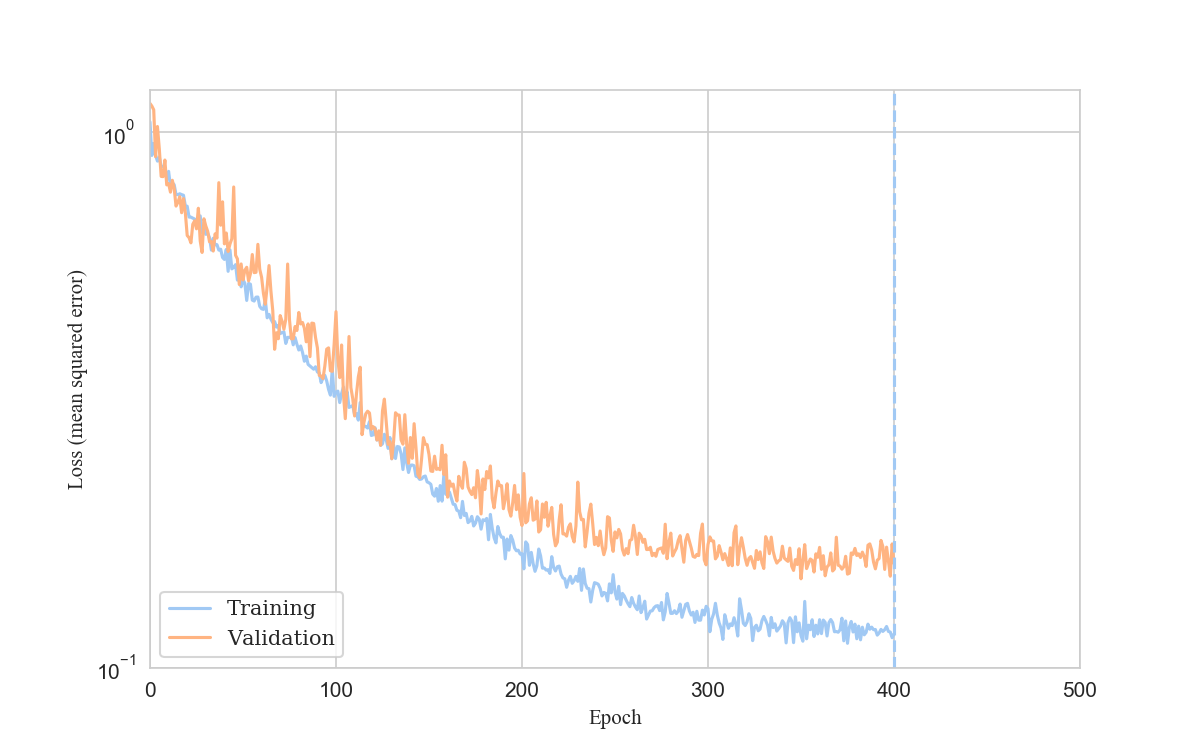
\includegraphics[width=\linewidth, keepaspectratio]{images/segm_history}
    \caption{Training history for the segmentation network. The y-axis represents the loss value (mean squared error). Both training and validation loss are plotted. The vertical dotted line indicates when early stopping occurred, due to a lack of improvement in the validation losse. Loss is expressed on a logarithmic scale.}
    \label{fig:segm_history}
  \end{center}
\end{figure}

\paragraph{Evaluation} The training process is visualized in figure \textcolor{blue}{\ref{fig:segm_history}}. The graph suggests that some improvement was still possible, but overtraining would become a real risk. Figure \textcolor{blue}{\ref{fig:segm_prediction}} shows how the network segmented a random selection of (previously unseen) test images. The model appears to yield acceptable results, especially given the very limited amount of training images it could work with. The average \textit{mean squared error} loss for each of the datasets is shown in table \textcolor{blue}{\ref{tab:segm_eval}}, along with the average \textit{dice loss}. The table indicates that the model is better accustomed to the training data, without being overly biased towards the validation images.

\begin{figure}[!htbp]
  \begin{center}
    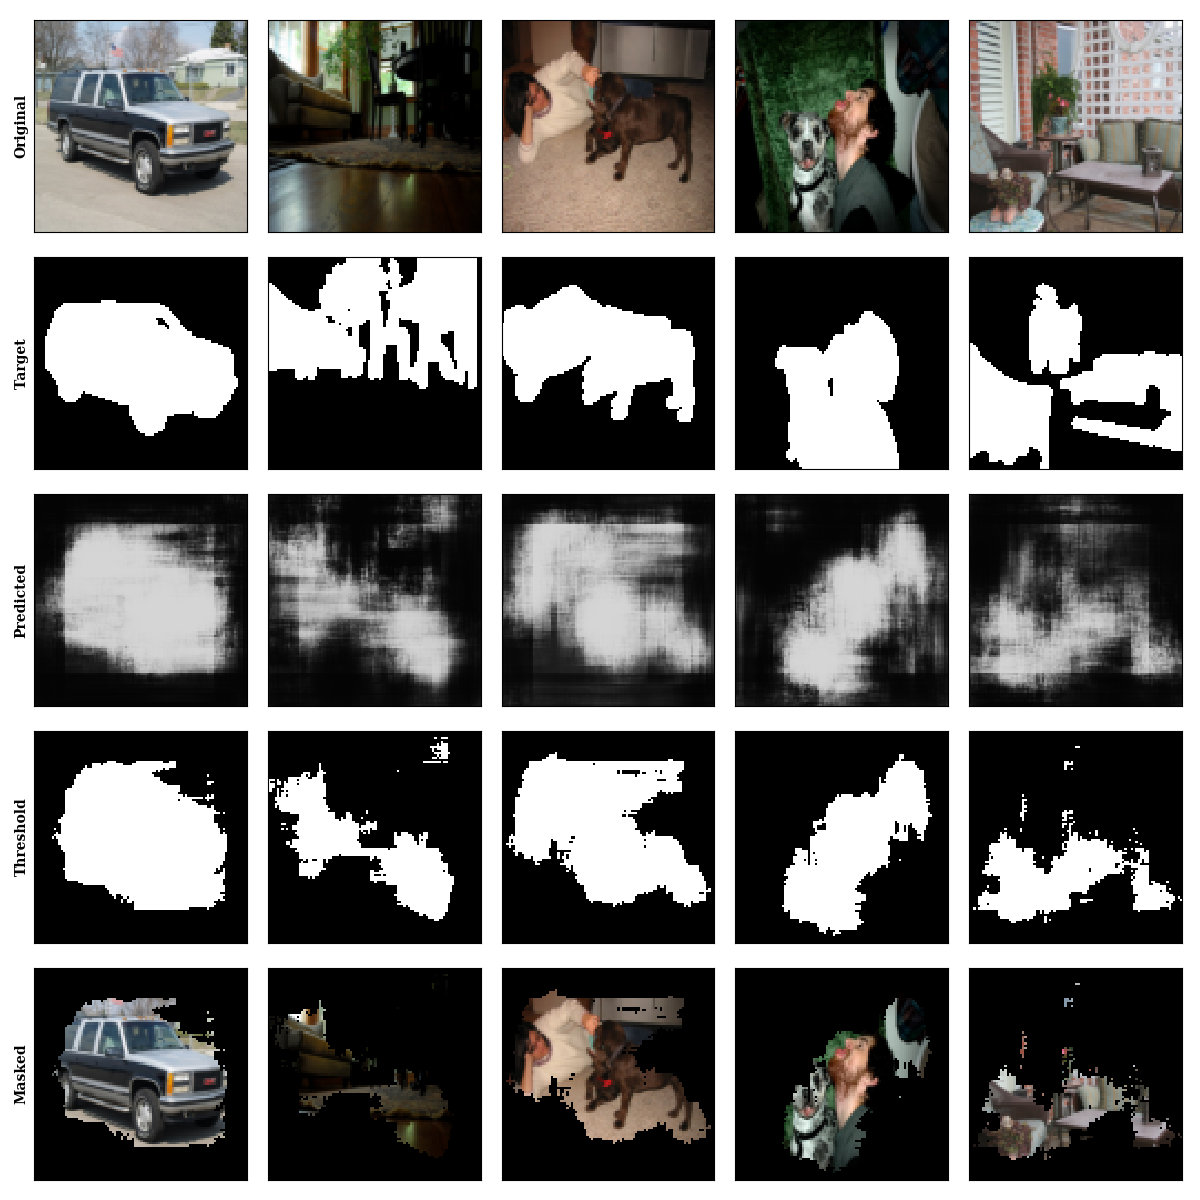
\includegraphics[width=\linewidth, keepaspectratio]{images/segm_prediction}
    \caption{Segmentation given by network for a random selection of 5 'fresh' test images ($96\times96\times3$ pixels). The top row shows the original images. The second row shows the binarized segmentation labels. The middle row shows the model output for the source images. The second to last row shows binarized predictions (threshold = $0.5$). The bottom row, finally, uses the binarized prediction as a mask over the source image.}
    \label{fig:segm_prediction}
  \end{center}
\end{figure}


\begin{table}[!htbp]
  \renewcommand{\arraystretch}{1.5}
  \centering

\begin{tabular}{@{}ccccc@{}}
\toprule
Model base                        & Loss                        & \textbf{Train} & \textbf{Validation} & \textbf{Test} \\ \midrule
\textit{\textbf{Autoencoder}}   & \textit{MSE} & \num{9.32e-2}  & \num{1.50e-1}       & \num{1.43e-1} \\
                              & \textit{Dice loss}          &                &                   &                \\
\textit{\textbf{U-Net}} & \textit{MSE} & \num{1.34e-1} & \num{1.39e-1}  & \num{1.50e-1}               \\
                              & \textit{Dice loss}          &   \num{5.80e-1}             & \num{6.00e-1}                     &  \num{5.94e-1}          \\ \bottomrule
\end{tabular}
  \caption{Evaluation of segmentation models using \textit{mean squared error (MSE)} and \textit{dice loss} values for training, validation and test datasets.}
  \label{tab:segm_eval}
\end{table}




% U-Net-based architecture %
%%%%%%%%%%%%%%%%%%%%%%%%%%%%


\subsection{U-Net-based segmentation network}

\begin{figure}[!htbp]
  \begin{center}
    \includegraphics[height=18cm, keepaspectratio]{images/segm_unet_architecture}
    \caption{U-Net-based architecture for the second segmentation network. Input dimensions are $96 \times 96 \times 3$. Output dimensions are $96 \times 96 \times 1$.}
    \label{fig:segm_unet_architecture}
  \end{center}
\end{figure}

In an effort to improve segmentation results, a second segmentation network was built. This time, the architecture was derived from U-Net---the convolutional network proposed for the purpose of biomedical image segmentation.

\paragraph{Architecture} 
The second segmentation model's architecture is shown in figure \ref{fig:segm_unet_architecture}. It is slightly more convoluted compared to the previous model, but still relatively simple. The so-called \textit{skip connections} mentioned in the assignment text can be seen, departing from every other convolutional layer to a 'partner' convolutional layer, thus helping the model to fine-tune its results in an early stage.

\paragraph{Network parameters} The model was trained using the same strategy as described in section \ref{sec:segm_1}. Image dimensions were kept the same, which is possible due to the dimension-agnostic nature of the U-Net architecture. The \textit{Adam} optimizer was used in training, in combination with \textit{mean squared error} loss. The total number of \textit{training epochs} was set to 500, and \textit{early stopping} occurred when improvement in the validation loss was absent for 50 epochs.

\begin{figure}[!htbp]
  \begin{center}
    \includegraphics[width=\linewidth, keepaspectratio]{images/segm_unet_prediction}
    \caption{Segmentation given by U-Net-based mdoel for a random selection of 5 'fresh' test images ($96\times96\times3$ pixels). The top row shows the original images. The second row shows the binarized segmentation labels. The middle row shows the model output for the source images. The second to last row shows binarized predictions (threshold = $0.5$). The bottom row, finally, uses the binarized prediction as a mask over the source image.}
    \label{fig:segm_unet_prediction}
  \end{center}
\end{figure}

% TODO: adjust!
\paragraph{Evaluation} Figure \textcolor{blue}{\ref{fig:segm_history}} shows the training history. The average \textit{mean squared error} loss for each of the datasets is shown in table \textcolor{blue}{\ref{tab:segm_eval}}, along with the average \textit{dice loss}. The table indicates that the model is better accustomed to the training data, without being overly biased towards the validation images. Some segmentation examples (on test images) are shown in figure \ref{fig:segm_unet_prediction}.



\subsection{Reflection}

\paragraph{Possible enhancement strategies} While the segmentation network described here has its merits, it is obviously far from perfect. Depending on the actual purpose of the network, additional operations could be applied to get the most out of the results. Should the problem be reframed as a detection problem (i.e., there is one object in the foreground: find it!), then it could suffice to find the center of the predicted foreground pixels and draw a rectangle around them (of which the dimensions are again based on the output activation).

If the objective is to extract the foreground object (by using the prediction as mask), this can be done more effectively by combining the network results with edge detection algorithms and morphological operations. The former may help create a better, more sensible outline for the detected foreground object(s). The latter may help in, for instance, filling in gaps, or generally smoothing out the result.

\begin{figure}[!htbp]
  \begin{center}
    \includegraphics[width=\linewidth, keepaspectratio]{images/segm_observation}
    \caption{This picture shows three purposely selected training images, along with their target, predicted, and thresholded segmentations, to illustrate apparent model strategizing attempts.}
    \label{fig:segm_observation}
  \end{center}
\end{figure}

\paragraph{Observation} While observing the output generated by the network, some interesting observations could be made. Sometimes the model makes mistakes in such a way that it shows its attempts at creating a generalizable strategy. More specifically, we can see how the model searches for distinct features such as edges, color differences, etc.
	
	Consider figure \ref{fig:segm_observation}. The first image (the bird sitting on the wire) came accompanied by a segmentation image that highlighted the bird, and nothing else. The model, on the other hand, shows tentative activation of the pixels in and around the wire. This 'mistake' is in fact rather intuitive, as the position of the wire is at about the same depth as the bird (the bird is setting the wire, after all). It can therefore be considered 'foreground' without much argument, suggesting that the model attempted to override the somewhat 'erroneous' labeling it was given. Similarly, for the second image, the model highlights the structure on the right on top of the bird. This is again a fairly forgivable mistake, as the structure appears to be quite distinct from the background, making it foreground by virtue of the problem's binary nature. The third image, finally, shows how these strategies can in some cases lead to errors that are not as easily classified as 'better judgment of the model'. Here, we see a discoloration in the background, due to a rock or gravel heap. This element is of course still in the background---something that is rather clear for a human observer. Due to its distinct visual features, however, the model mistakenly tries to add it to the foreground. 
	
	Importantly, all the images shown here are training images. The mistakes made here persisted despite numerous chances for the model to adjust for them. They are thus inherently linked with the model's attempt at learning a strategy.

% Interesting: picture of training 